\section{Backend Capacity Planning} \label{sec:theory}




     

\subsection{Backend Capacity Optimization}\label{sec:plan}

Without loss of generality, we define the backend capacity as the maximum number of requests that can be served per minute, which is directly linked to the cost of the backend (e.g., to pay for the MBaaS service plan or the instances on Amazon EC2). We assume that the developer is able to adjust the backend capacity on an hourly basis. Let $N$ denote the required backend capacity, to be determined by the optimization model. The developer classifies all possible requests of the application into $K$ types, according to their delay tolerance. For example, there can be $K=3$ types of requests: urgent, medium, and delay-tolerant. An hour consists of $i = 1,2,...,60$ minutes, during which the backend capacity is fixed. Let $n_i^k$ denote the estimated number of type $k$ requests that will arrive at the $i$-th minute in the next hour. In this section, we assume that  $n_i^k, i\in[1,60], k \in[1,K]$ are available as inputs to the optimization model, and we will discuss how to predict $n_i^k$ in details in the next section. Without Clockwork, to guarantee the performance of the backend, the developer has to make sure that the backend capacity is greater than the peak demand, i.e., $N \ge \max_i\sum_k n_i^k$. We will show that such over-provisioning is unnecessary with the request scheduling mechanism of Clockwork.  


We make the simplified assumption that all requests generated in a specific hour will be served within that hour. In other words, during the current hour, the backend will neither serve requests from the previous hour, nor put off requests to the next hour. At the $i$-th minute, let $\delta_{ij}^k \in [0,1]$ denote the proportion of the $n_i^k$ requests that will be postponed to the $j$-th minute. We have $i \le j \le 60$, and $\delta_{ii}^k$ is the proportion of requests that are not delayed.  All requests to be served at the $j$-th minute, denoted by $N_j$, include those deferred from the previous minutes to the $j$-th minute, and those generated and instantly served in the $j$-th minute, i.e., $N_j = \sum_{i=1}^{j-1}\sum_{k=1}^K\delta_{ij}^k n_i^k + \sum_{k=1}^K\delta_{jj}^k n_j^k = \sum_{i=1}^{j}\sum_{k=1}^K\delta_{ij}^k n_i^k$. To guarantee the performance of the backend, its capacity should be larger than the peak demand after request scheduling, i.e., $N \ge \max_{j\in[1,60]}N_j$. 

Delaying requests will affect the user experience, thus the developer needs to have a control over how many and how long a certain type of requests can be delayed. Clockwork allows the developer to set the upper-bound of $\delta_{ij}^k$ as $\overline{\delta_{ij}^k}$, which depends on the request  type $k$ and the length of delay $j-i$. For instance, in a social messaging application, if  \emph{sending a message} is regarded as the most urgent type of requests and should not be delayed, the developer can simply set $\forall j > i,\overline{\delta_{ij}^{\textrm{send a message}}} = 0$; if no request should be delayed for more than half an hour, the developer can simply stipulate that $\forall k,\overline{\delta_{ij}^{k}} = 0, \textrm{if } j - i > 30$.     

As the backend cost will monotonically increase with the backend capacity, we set the objective of Clockwork as to minimize the required backend capacity, without violating the constraint on $\delta_{ij}^k$ designated by the developer.

\begin{align}\label{equ:opt}
\min\limits_{\delta_{ij}^k}~ & N, \\
\textrm{subject to } & N \ge \max\limits_{j\in[1,60]}N_j, \label{equ:constraint0}\\
& N_j = \sum_{i=1}^{j}\sum_{k=1}^K\delta_{ij}^k n_i^k, \forall j,\label{equ:constraint1}\\
&\sum\limits_{j = i}^{60} \delta_{ij}^k = 1, \forall i, \forall k,\label{equ:constraint}\\
& 0\le \delta_{ij}^k \le \overline{\delta_{ij}^k}, \forall i, \forall j, \forall k.
\end{align}
Constraint (\ref{equ:constraint0}) guarantees that the backend capacity is large enough to meet the peak request demand. Constraint (\ref{equ:constraint1}) shows the number of requests per minute after scheduling. Constraint (\ref{equ:constraint}) ensures that all the requests initiated in the $i$-th minute are served, either instantly or in later minutes. The objective function is minimized through variables $\delta_{ij}^{k}$, and we can get the optimal backend capacity as $N^*  = \max_{j\in[0,60]}N_j^*$, in which $N_j^* = \sum_{i=1}^{j}\sum_{k=1}^K{\delta_{ij}^k}^* n_i^k$. The optimization problem (\ref{equ:opt}) is a linear programming problem, and can be solved by existing algorithms such as Simplex and Interior point algorithms. Fig.~\ref{fig:serviceplan2} gives an example of how the backend capacity planning of Clockwork works. It is shown that the demand profile is smoothed as Clockwork schedules requests to \emph{cut} the peak and \emph{fill} the valley.   



\begin{figure}[t]
	\center
	\hspace{-0.2cm}
	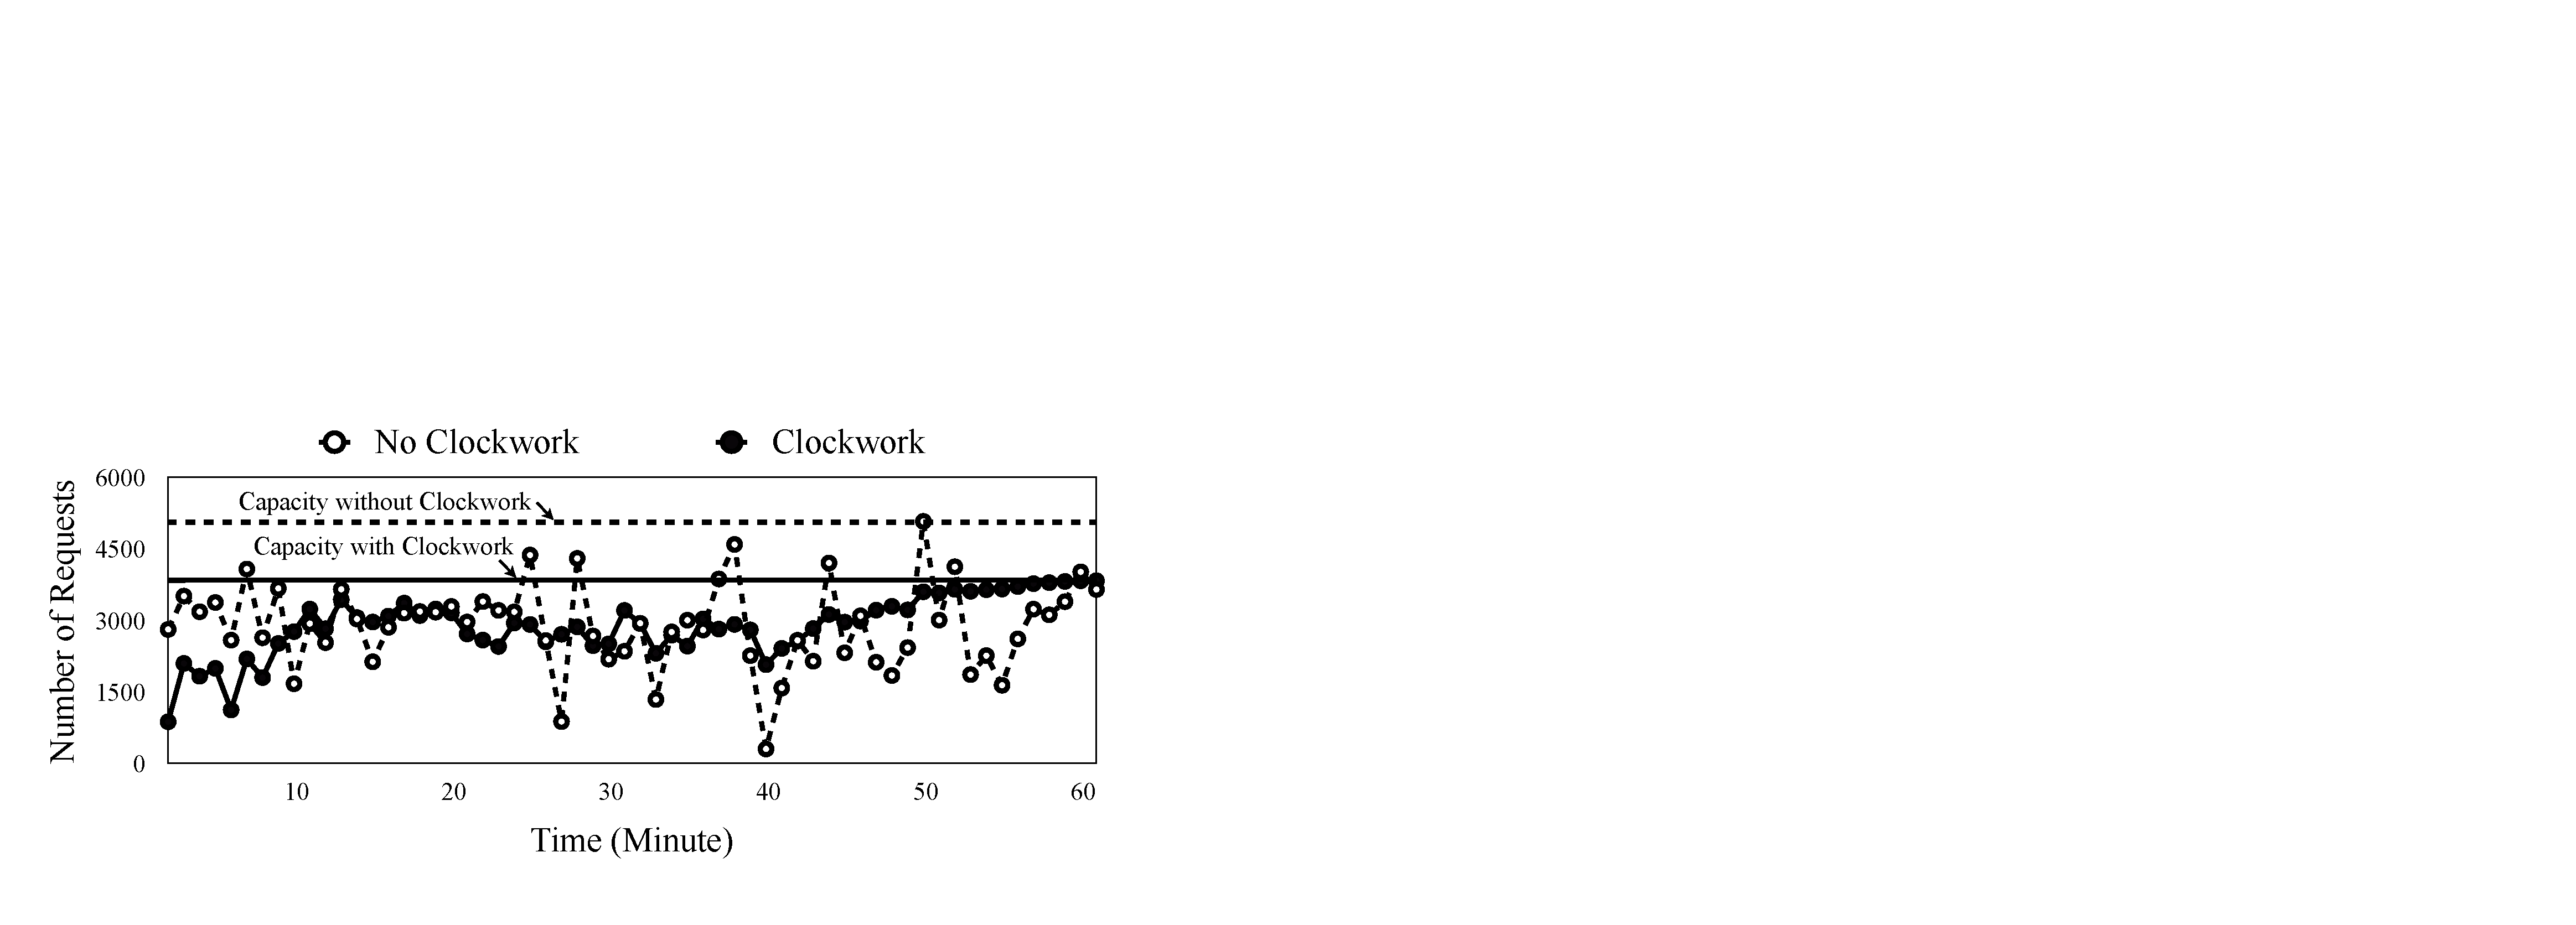
\includegraphics[trim = 0mm 0mm 0mm 0mm,clip,width=3.3in]{figs/cp1}
	\caption{Request demand smoothing by Clockwork.} \label{fig:serviceplan2}
\end{figure}	

\subsection{Future Demand Prediction}\label{sec:predict}

The optimization problem (\ref{equ:opt}) requires the input of $n_i^k$, the expected number of type $k$ requests generated at the $i$-th minute of the next hour, which can be learned from historical data using machine learning algorithms.  We focus on four widely-used  algorithms: logistic regression (LR), single-hidden-layer multilayer perceptron (sMLP), deep belief networks (DBN), and convolutional neural networks (CNN). Logistic regression and sMLP are simple machine learning models, while DBN and CNN are deep learning models. For simplicity, in this paper, we use these models for classification, while they can easily be adapted for regression. For instance, $n_i^k\in (1,100]$ and $n_i^k \in (100, 200]$ can be defined as class $1$ and class $2$, respectively. 

Historical data are collected in the form of the number of requests generated in each minute. The input vector $\pmb{x}$ to the machine learning model should contain the best predictors for $n_i^k$. Two potential factors need to be taken into consideration. One is \emph{temporal-proximity}, i.e., the most recent demand indicates the near future. The other is \emph{diurnal} effect, i.e., demands at the same time of each day have a similar trend. Therefore, we use the demand of the previous two hours and the demand at the same time of the previous two days as the input vector to predict $n^k_i$, i.e., $\pmb{x}=(n_{i-180}^k,\cdots, n_{i-61}^k, n_{i-1440-180}^k,\cdots,n_{i-1440+179}^k,\\ n_{i-1440*2-180}^k,\cdots n_{i-1440*2+179}^k)$, and $Y= n^k_i$. Furthermore, we normalize entries in the input vectors as $\pmb{x} \rightarrow \pmb{x}/\max\{n_i^k\}$, and discretize the output into $10$ levels for classification.  

We use synthetic datasets to evaluate the performance of the four machine learning models as follows. Assume that there are $100$ users, each generating requests according to a Poisson process. Without loss of generality, we only consider one type of requests. We first generate a series of values with a diurnal pattern (low demand at working time, and high demand at leisure time), to represent the request arrival rate at different time of a day for an average user. Then, we compute the arrival rate for each individual user by adding noise to the arrival rate of the average user. Aggregating the number of requests from all users at each minute yields the demand profile. We run the four machine learning algorithms on a MacBook Pro laptop with $2.9$ GHz Intel CPU and 8 GB memory.     


\begin{figure}[t]
	\center
	\hspace{-0.4cm}
	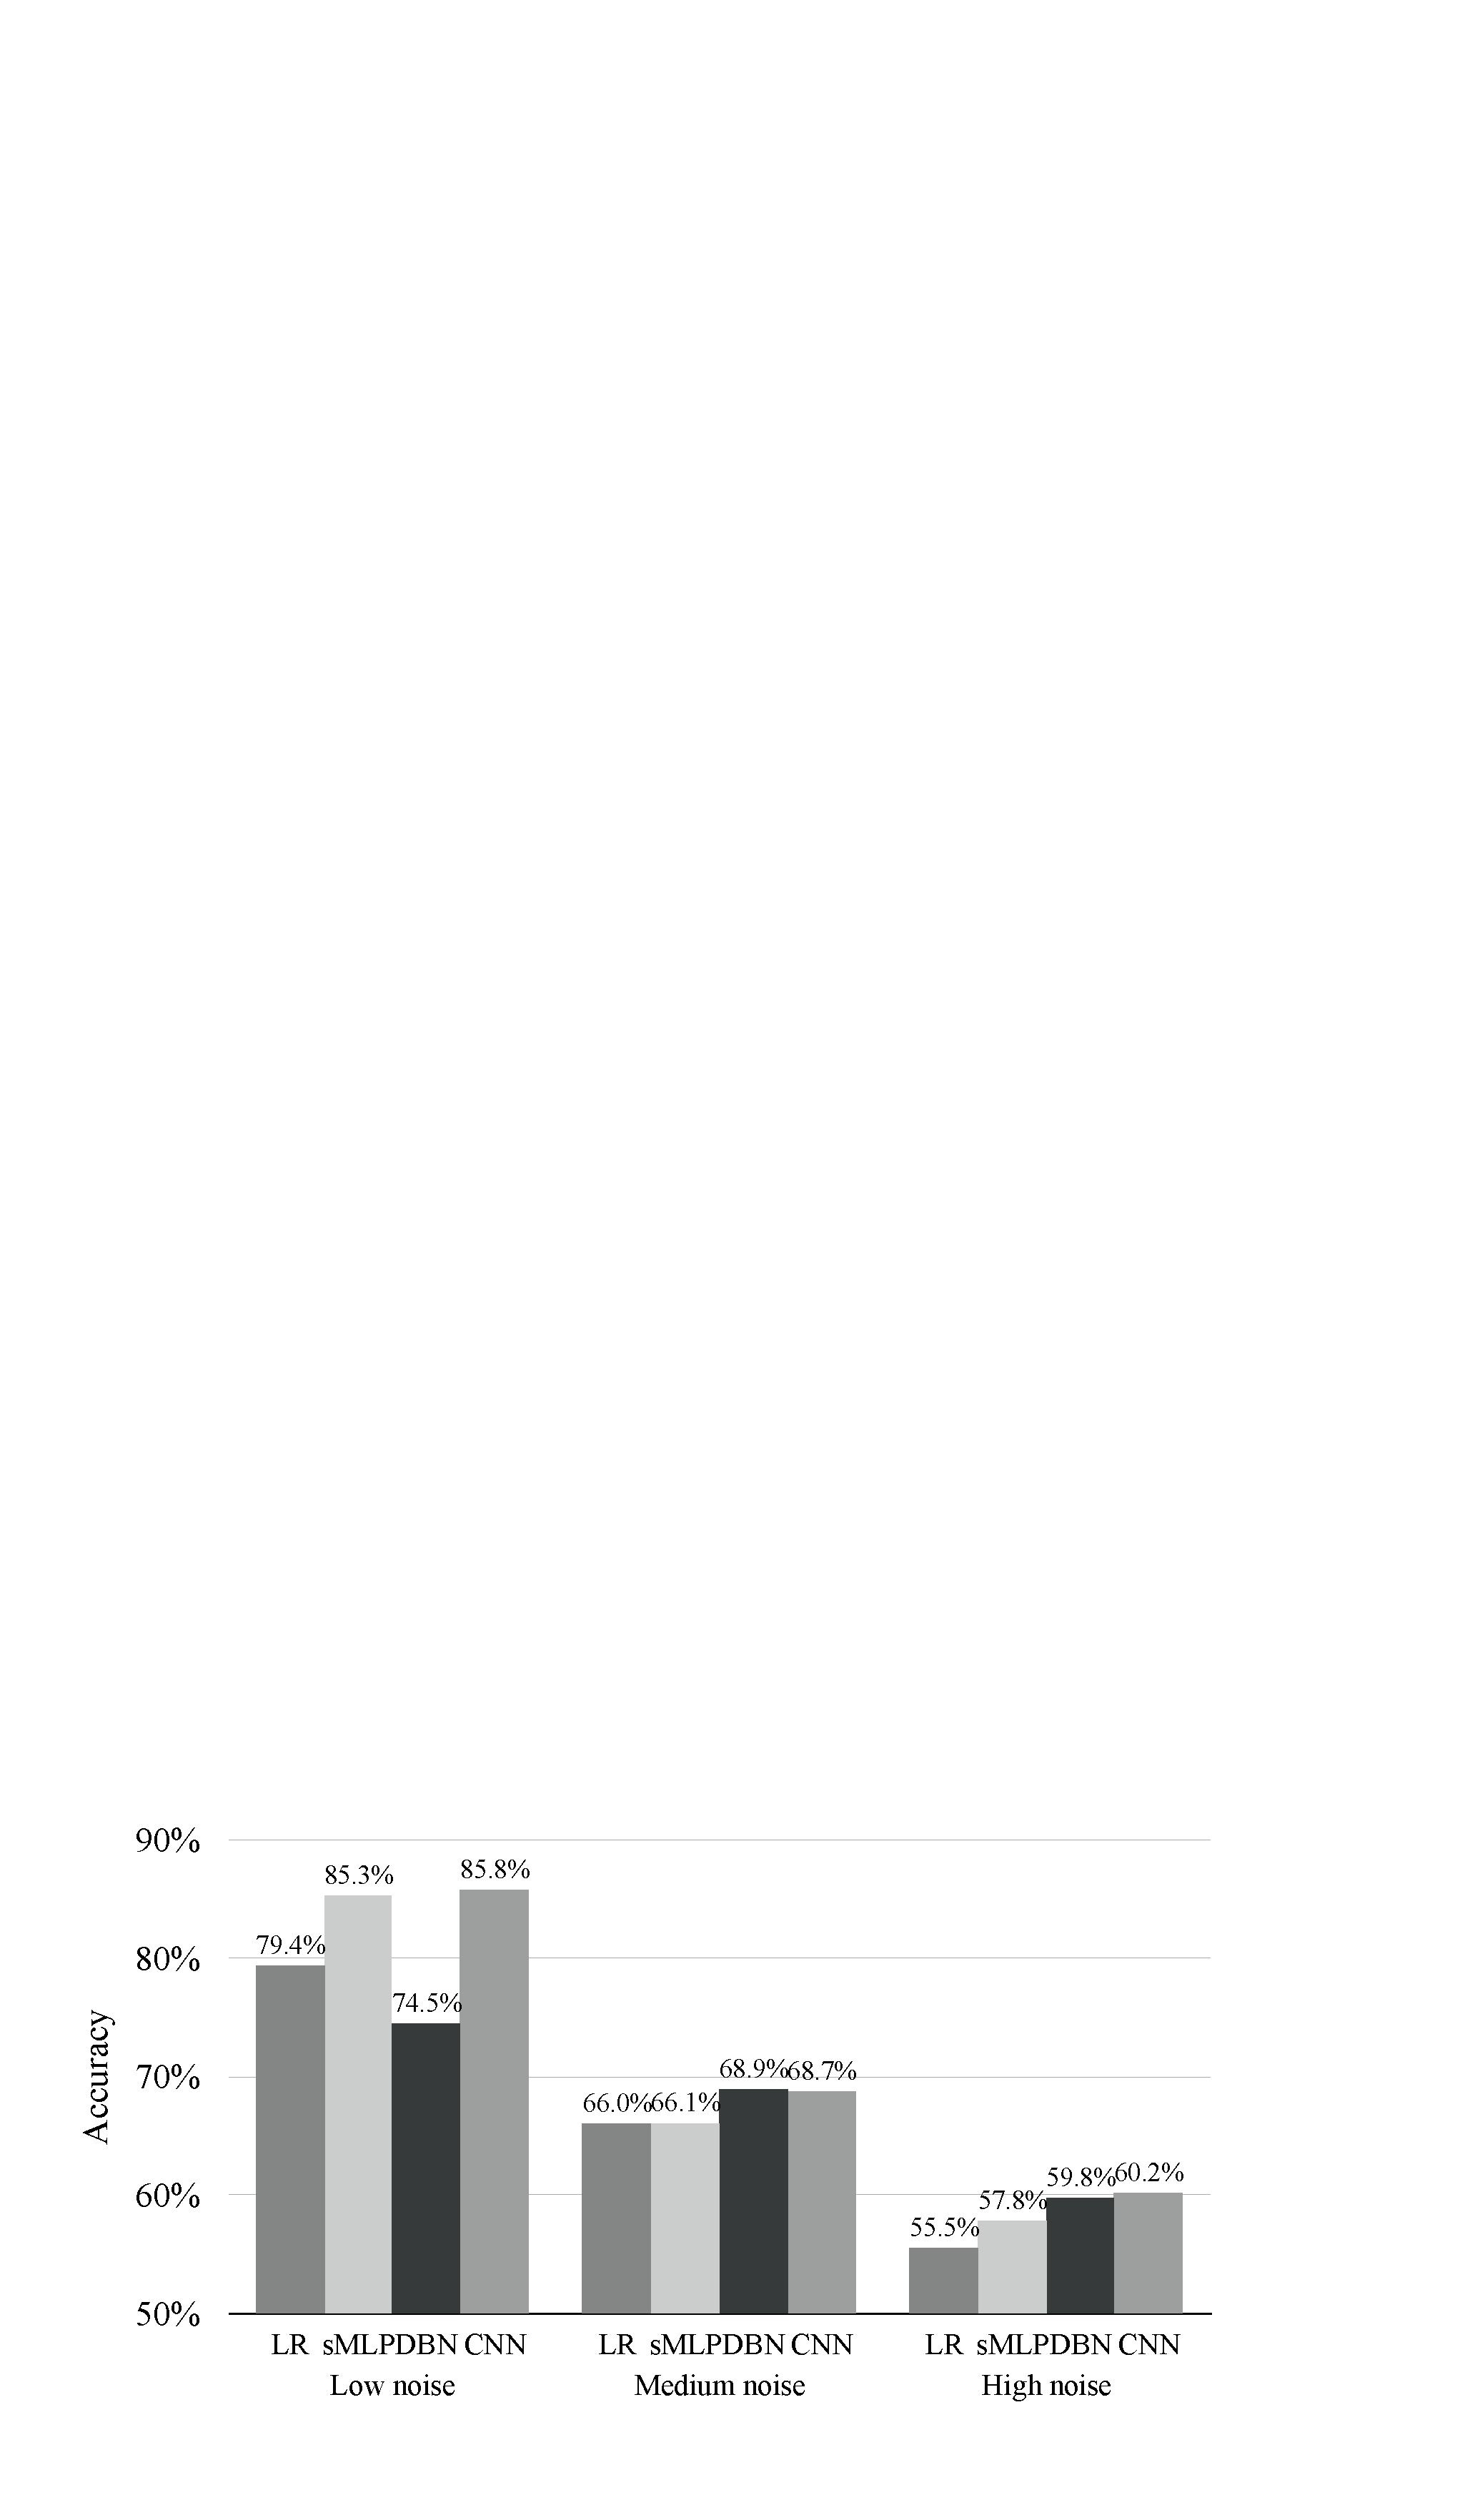
\includegraphics[trim = 0mm 0mm 0mm 12mm,clip,width=3.4in]{figs/acc}
	\caption{Prediction accuracy.} \label{fig:acc}
\end{figure}

As shown in Fig.~\ref{fig:acc}, deep learning models outperform simple models when the dataset is more noisy, since deep learning models are more powerful in discovering the intricate relationship between the input and the output. Unexpectedly, at the low noise level, DBN gives the worst prediction result, even inferior to the logistic regression model. One possible reason is that the complicated structure of DBN leads to the over-fitting problem. In other words, the model exaggerates the noise in the training data, instead of learning the general trend, therefore gives poor predictions when applied to the testing data. 

As shown in Fig.~\ref{fig:time}, the training time of deep learning models is far higher than that of simple models, which is not surprising since the deep learning models contain far more parameters to be learned. The training time of DBN and CNN also depends on the choice of the number of layers and neurons in each layer. Though the training time diverges considerably, given a new input, it takes almost the same time (less than a second) for the trained models of all four algorithms to yield the prediction result. 


\begin{figure}[t]
	\center
	\hspace{-0.4cm}
	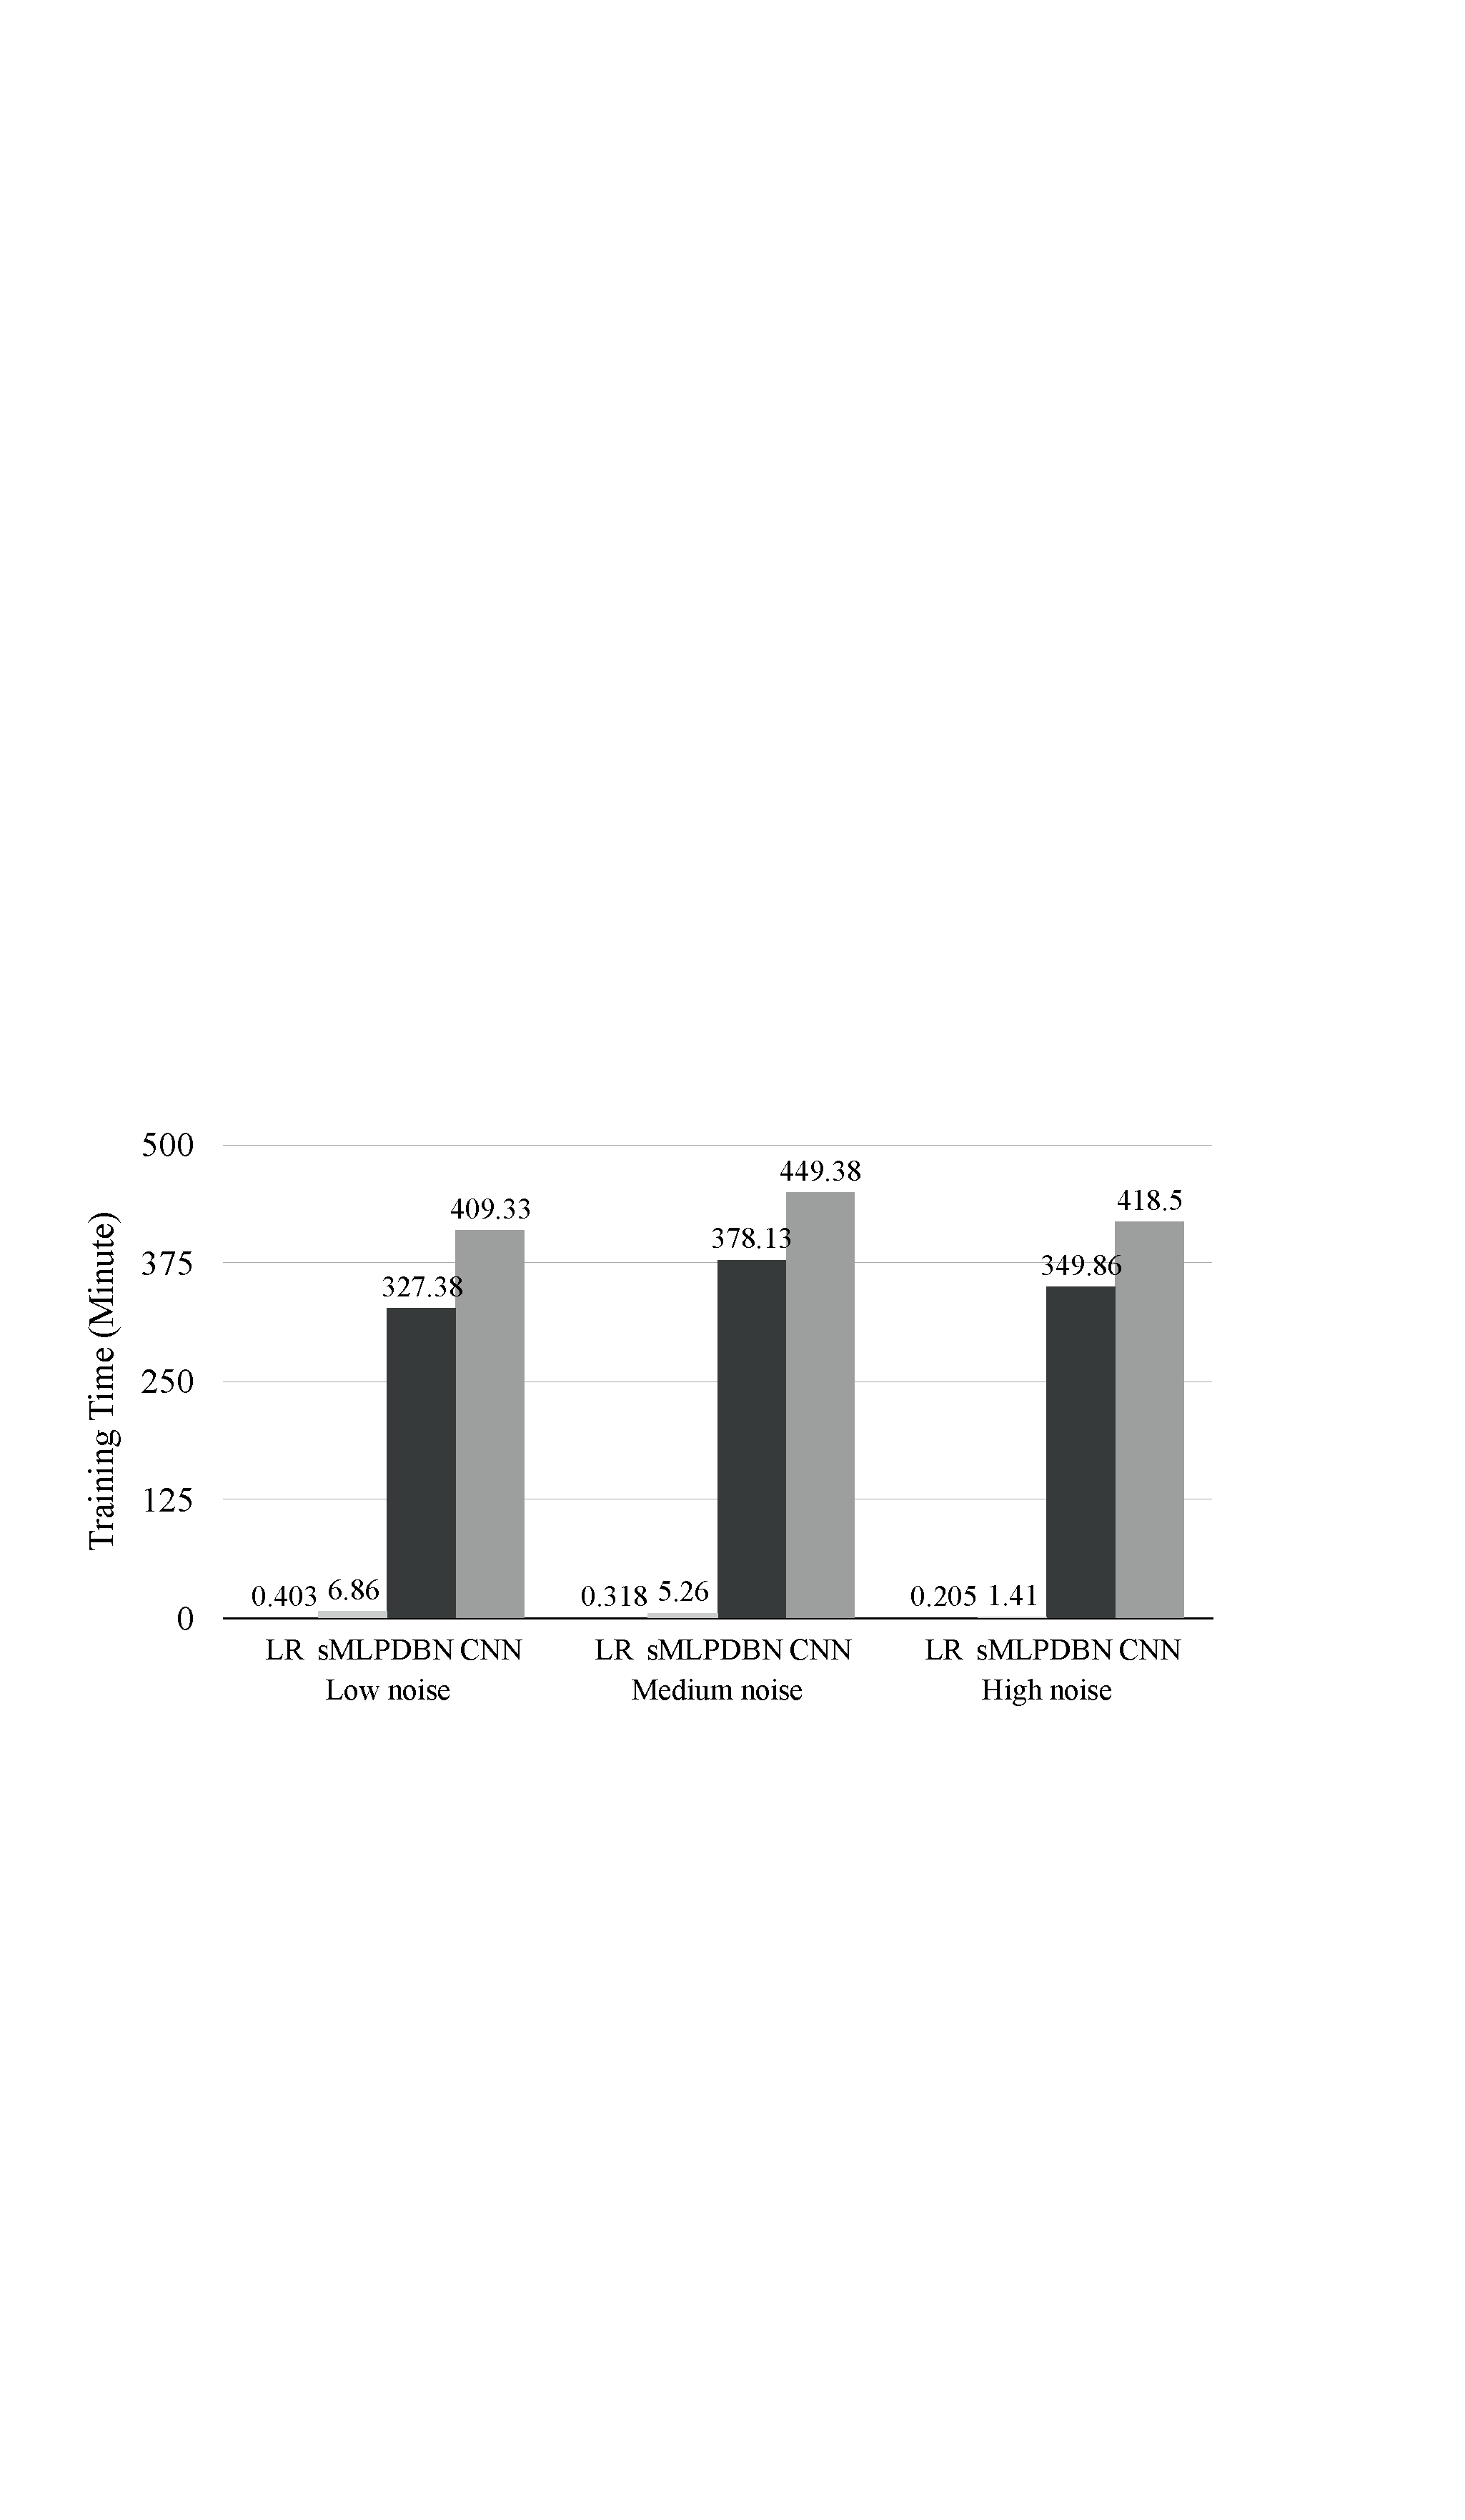
\includegraphics[trim = 0mm 0mm 0mm 12mm,clip,width=3.4in]{figs/t}
	\caption{Training time.} \label{fig:time}
\end{figure}  

 

